\chapter{พื้นฐานฟิสิกส์เชิงแสงและสรีรวิทยาของสีดิน}
\label{ch:foundations}

\section{บทนำและหลักการฟิสิกส์ของการสะท้อนแสงบนพื้นผิวดิน}

การประเมินสถานะความสมบูรณ์ของดินด้วยวิธีการทางแสง (Optical Soil Sensing) มีรากฐานสำคัญมาจากฟิสิกส์ของการแผ่รังสีแม่เหล็กไฟฟ้า (Electromagnetic Radiation) และการกระเจิงแสงแบบพร่ากระจาย (Diffuse Reflectance) บนตัวกลางที่มีความไม่ต่อเนื่องเชิงจุลภาค เมื่อลำแสงตกกระทบลงบนผิวตัวอย่างดินที่มีความขรุขระ รังสีส่วนหนึ่งจะเกิดการสะท้อนที่ผิวสัมผัสภายนอก (Specular Fresnel Reflection) ในขณะที่รังสีส่วนใหญ่จะทะลวงผ่านเข้าไปในเนื้อดิน เกิดการหักเห การกระเจิงซ้ำไปมาหลายทิศทาง (Multiple Scattering) และการดูดกลืนพลังงานบางส่วนโดยโมเลกุลของสสารภายในดิน ก่อนจะแผ่ย้อนกลับออกมาสู่พื้นผิวเป็นรังสีสะท้อนพร่ากระจาย ซึ่งสามารถจำลองปรากฏการณ์ดังกล่าวได้ด้วยทฤษฎีคูเบลกา--มังก์ (Kubelka--Munk Theory) ดังสมการ

\begin{equation}
\frac{K}{S} = \frac{(1 - R_\infty)^2}{2 R_\infty}
\label{eq:kubelka_munk}
\end{equation}

โดยที่ $K$ คือสัมประสิทธิ์การดูดกลืนแสงเชิงโมลาร์ (Absorption Coefficient) $S$ คือสัมประสิทธิ์การกระเจิงแสงของเม็ดดิน (Scattering Coefficient) และ $R_\infty$ คือสภาพสะท้อนแสงของชั้นดินที่มีความหนามากจนแสงไม่ทะลุผ่าน (Infinite Thickness Reflectance)

สารประกอบหลักในดินที่มีบทบาทสำคัญอย่างยิ่งต่อการกำหนดลักษณะของค่า $K$ ในช่วงความยาวคลื่นแสงที่ตามองเห็น (Visible Spectrum ความยาวคลื่น 380 ถึง 750 นาโนเมตร) ได้แก่ อินทรียวัตถุในดิน (Soil Organic Matter หรือ SOM) ซึ่งประกอบด้วยกรดฮิวมิก (Humic Acid) และกรดฟุลวิก (Fulvic Acid) สารประกอบกลุ่มนี้มีโครงสร้างวงแหวนอะโรมาติกขนาดใหญ่ที่มีระบบพันธะคู่คู่ควบ (Conjugated $\pi$-electron Systems) จำนวนมาก ทำให้เกิดแถบการดูดกลืนแสงที่กว้างขวางครอบคลุมทั่วทั้งสเปกตรัม ส่งผลให้ดินที่มีอินทรียวัตถุสูงปรากฏเป็นสีน้ำตาลเข้มจนถึงดำสนิท

นอกจากนี้ แร่เหล็กออกไซด์ (Iron Oxides) เช่น เกอไทต์ ($\alpha\text{-FeOOH}$) จะแสดงแถบการดูดกลืนแสงเด่นชัดในช่วงคลื่นสีน้ำเงิน (400 ถึง 450 นาโนเมตร) เนื่องจากกระบวนการถ่ายโอนประจุระหว่างลิแกนด์กับโลหะ (Ligand-to-Metal Charge Transfer) และการเปลี่ยนสถานะทางอิเล็กตรอนของไอออน $\text{Fe}^{3+}$ ในโครงผลึกแปดหน้า (Octahedral Crystal Field Transition) ทำให้สะท้อนแสงช่วงสีเหลืองและน้ำตาลส้ม ในขณะที่ฮีมาไทต์ ($\alpha\text{-Fe}_2\text{O}_3$) มีแถบการดูดกลืนที่ขยับไปทางความยาวคลื่นที่ยาวกว่า จึงสะท้อนแสงช่วงสีแดงสดอย่างเด่นชัด

\begin{theorybox}
\textbf{ฟิสิกส์การดูดกลืนแสงของหมู่โมเลกุลในเนื้อดิน}\par
การแปรผันของความสว่าง (Luminance หรือ $L^*$) ในเนื้อดินเป็นฟังก์ชันผกผันโดยตรงกับปริมาณอินทรียวัตถุในดิน ($C_{\text{SOM}}$) ตามกฎของเบียร์--แลมเบิร์ตเชิงขยาย (Extended Beer--Lambert Law) เมื่อตัวอย่างดินมีความชื้นสม่ำเสมอ ความเข้มแสงสะท้อนที่ตรวจจับได้จากเซนเซอร์รับภาพดิจิทัล ($I_{\text{reflected}}$) สามารถเชื่อมโยงทางคณิตศาสตร์ได้ดังนี้
\begin{equation}
I_{\text{reflected}}(\lambda) = I_0(\lambda) \cdot \exp\left( - \left[ \alpha_{\text{SOM}}(\lambda) C_{\text{SOM}} + \sum_i \alpha_i(\lambda) C_i \right] \cdot d_{\text{path}} \right)
\end{equation}
โดย $I_0(\lambda)$ คือความเข้มแสงตกกระทบจากหลอดกำเนิดแสงมาตรฐาน $\alpha_{\text{SOM}}(\lambda)$ คือสภาพดูดกลืนแสงจำเพาะของอินทรียวัตถุ และ $d_{\text{path}}$ คือระยะทางเฉลี่ยที่โฟตอนเดินทางกระเจิงอยู่ในช่องว่างระหว่างเม็ดดิน
\end{theorybox}

\section{เคมีฟิสิกส์ของปฏิกิริยาสีอินดิเคเตอร์วัดความเป็นกรดด่าง}

การตรวจวัดระดับความเป็นกรดด่างของดินด้วยสายตาหรือคอมพิวเตอร์วิทัศน์ มักดำเนินการผ่านกระบวนการสกัดสารละลายดิน (Soil Suspension Extraction) โดยใช้น้ำปราศจากไอออนหรือสารละลายโพแทสเซียมคลอไรด์ร่วมกับสารละลายอินดิเคเตอร์ผสม (Universal Indicator Formulation) ซึ่งอาศัยหลักการเปลี่ยนรูปทางโครงสร้างเคมีและการเปลี่ยนระดับพลังงานของโมเลกุลโครโมฟอร์ (Chromophore) เมื่อรับหรือปลดปล่อยโปรตอน ($\text{H}^+$)

พิจารณาสมดุลกรดเบสของสารอินดิเคเตอร์ชนิดโบรโมไทมอลบลู (Bromothymol Blue) และเมทิลเรด (Methyl Red) ในระบบสารละลาย ดังสมการ

\begin{equation}
\text{H}\text{Ind} \rightleftharpoons \text{H}^+ + \text{Ind}^-
\end{equation}

ค่าคงที่การแตกตัวของอินดิเคเตอร์ ($K_a$) กำหนดอัตราส่วนความเข้มข้นระหว่างรูปกรดและรูปเบสตามสมการแฮนเดอร์สัน--ฮัสเซลบัลค์ (Henderson--Hasselbalch Equation)

\begin{equation}
\text{pH} = \text{p}K_a + \log_{10}\left( \frac{[\text{Ind}^-]}{[\text{H}\text{Ind}]} \right)
\label{eq:henderson}
\end{equation}

เมื่อสารละลายดินมีสภาวะเป็นกรดจัด ($\text{pH} < 5.0$) อินดิเคเตอร์จะคงอยู่ในรูป $\text{H}\text{Ind}$ ซึ่งดูดกลืนแสงช่วงสีน้ำเงินและเขียวอย่างรุนแรง ส่งผลให้แสงสะท้อนที่ตามองเห็นปรากฏเป็นเฉดสีแดงและส้มเหลือง เมื่อค่า $\text{pH}$ เพิ่มสูงขึ้นสู่สภาวะเป็นกลางและด่าง ($\text{pH} > 7.0$) โมเลกุลจะปลดปล่อยโปรตอนกลายเป็นรูปประจุลบ $\text{Ind}^-$ การจัดเรียงตัวของวงแหวนคอนจูเกชันเปิดกว้างขึ้น ส่งผลให้ระดับพลังงานขั้นกระตุ้นลดต่ำลง ทำให้เกิดการดูดกลืนแสงช่วงสีเหลืองและแดง ส่งผลให้สารละลายสะท้อนคลื่นแสงช่วงสีเขียวตอง เขียวมรกต และน้ำเงินเข้มอย่างเด่นชัด การแปลงการเปลี่ยนแปลงทางสเปกตรัมนี้ให้อยู่ในรูปพิกัดสีดิจิทัลจึงทำให้คอมพิวเตอร์วิทัศน์สามารถประมาณค่า $\text{pH}$ ได้อย่างแม่นยำ

\section{สรีรวิทยาและเคมีสีของการวิเคราะห์ธาตุอาหารหลัก ไนโตรเจน ฟอสฟอรัส โพแทสเซียม}

การตรวจวัดธาตุอาหารหลักพืช N-P-K ด้วยวิธีการทางเคมีสี (Colorimetric Assay) ใช้อนุพันธ์ของปฏิกิริยาเคมีที่ให้สารประกอบเชิงซ้อนสีจำเพาะ (Specific Chromogenic Complexes) ซึ่งมีคุณลักษณะการดูดกลืนแสงแปรผันตรงกับความเข้มข้นของไอออนธาตุอาหาร ดังนี้

\subsection{ไนโตรเจนที่ใช้ประโยชน์ได้ (Available Nitrogen)}
ไนโตรเจนในดินส่วนใหญ่อยู่ในรูปไนเตรต ($\text{NO}_3^-$) และแอมโมเนียม ($\text{NH}_4^+$) ปฏิกิริยาการตรวจวัดไนเตรตอาศัยการรีดิวซ์ไนเตรตเป็นไนไตรต์ ($\text{NO}_2^-$) ด้วยผงสังกะสีหรือแคดเมียม จากนั้นเกิดปฏิกิริยาไดอะโซไทเซชัน (Griess Diazotization Reaction) กับสารซัลฟานิลาไมด์ (Sulfanilamide) และควบคู่กับแนฟทิลเอทิลีนไดอะมีน (N-(1-naphthyl)ethylenediamine) เกิดเป็นสารประกอบเชิงซ้อนสีย้อมเอโซ (Azo Dye) สีชมพูอมม่วงเข้ม ซึ่งมีความเข้มการดูดกลืนแสงสูงสุดที่ความยาวคลื่น 540 นาโนเมตร

\subsection{ฟอสฟอรัสที่เป็นประโยชน์ (Available Phosphorus)}
ฟอสฟอรัสในรูปออร์โทฟอสเฟต ($\text{H}_2\text{PO}_4^-$ และ $\text{HPO}_4^{2-}$) ทำปฏิกิริยากับแอมโมเนียมโมลิบเดต (Ammonium Molybdate) ภายใต้สภาวะกรดรุนแรง เกิดเป็นกรดฟอสโฟโมลิบดิก (Phosphomolybdic Acid) ซึ่งเมื่อถูกรีดิวซ์ด้วยกรดแอสคอร์บิก (Ascorbic Acid) จะเปลี่ยนโครงสร้างเป็นโมลิบดินัมบลู (Molybdenum Blue Complex) ที่มีสีน้ำเงินเข้ม การดูดกลืนแสงสูงสุดอยู่ที่ความยาวคลื่น 880 นาโนเมตร และมีหางสเปกตรัมครอบคลุมช่วงแสงสีแดงเข้ม (650 ถึง 700 นาโนเมตร) ทำให้การเปลี่ยนแปลงค่าพิกัดสีแดงและน้ำเงินในระบบ RGB และ CIE $L^*a^*b^*$ มีความสัมพันธ์เชิงฟังก์ชันอย่างเด่นชัด

\subsection{โพแทสเซียมที่แลกเปลี่ยนได้ (Exchangeable Potassium)}
โพแทสเซียมไอออน ($\text{K}^+$) ตรวจวัดด้วยการตกตะกอนร่วมกับโซเดียมเตตระฟีนิลโบเรต (Sodium Tetraphenylborate, $\text{NaB(C}_6\text{H}_5)_4$) เกิดเป็นตะกอนอนุภาคแขวนลอยสีขาวขุ่นของโพแทสเซียมเตตระฟีนิลโบเรต ($\text{KB(C}_6\text{H}_5)_4$) ซึ่งความขุ่นของสารละลายทำให้เกิดการกระเจิงแสงแบบเรย์ลี--ดีบาย (Rayleigh--Debye Scattering) การวัดระดับความขุ่นและเฉดสีเหลืองของรีเอเจนต์ร่วม ทำให้สามารถประเมินระดับความเข้มข้นของโพแทสเซียมจากค่าความสว่างสัมพัทธ์ได้อย่างแม่นยำ

\section{ข้อจำกัดของเซนเซอร์หัววัดไฟฟ้าแบบแทงดินและวิวัฒนาการสู่การตรวจวัดเชิงแสง}

หัววัดดินแบบอิเล็กโทรดเชิงโลหะ (Metallic Probe 7-in-1) อาศัยการวัดค่าการนำไฟฟ้าปรากฏ (Apparent Electrical Conductivity หรือ $\text{EC}_a$) ขั้วไฟฟ้ากระแสสลับความถี่สูง และความต่างศักย์รีดอกซ์ ซึ่งแม้จะสะดวกในการใช้งานภาคสนาม แต่พบข้อจำกัดทางฟิสิกส์ที่ไม่อาจหลีกเลี่ยงได้ ดังนี้

\begin{enumerate}[label=\textbf{\arabic*.}]
\item \textbf{ผลกระทบจากความต้านทานสัมผัส (Contact Resistance Variance)} แรงกดในการแทงหัววัดและความหนาแน่นรวมของดิน (Bulk Density) ส่งผลให้พื้นที่สัมผัสระหว่างผิวโลหะและเม็ดดินแปรปรวน นำไปสู่ความคลาดเคลื่อนของค่าที่อ่านได้สูงถึง $\pm 25\%$
\item \textbf{ผลกระทบจากการเจือปนของเกลือและความชื้น (Moisture-Salinity Cross-Interference)} การอ่านค่าไนโตรเจน ฟอสฟอรัส และโพแทสเซียมจากหัววัดไฟฟ้ามักเป็นการประมาณการทางอ้อมจากค่า $\text{EC}$ ทำให้เมื่อดินมีความชื้นแปรผันหรือมีเกลือสะสม หัววัดจะประเมินค่า N-P-K ผิดพลาดอย่างมีนัยสำคัญ
\item \textbf{การเกิดชั้นออกไซด์และการสึกกร่อน (Electrode Passivation)} การใช้งานหัววัดโลหะในดินที่มีสภาพกรดจัดอย่างต่อเนื่อง ก่อให้เกิดฟิล์มออกไซด์ที่ผิวโลหะ ทำให้ความไวในการตอบสนองลดลงตามระยะเวลา
\end{enumerate}

ด้วยเหตุนี้ การบูรณาการเทคโนโลยีคอมพิวเตอร์วิทัศน์และโมเดลการเรียนรู้เชิงลึกเข้ามาร่วมวิเคราะห์ จึงช่วยสร้างระบบถ่วงดุลสองทิศทาง (Bimodal Cross-Verification) โดยนำคุณลักษณะทางแสงที่สะท้อนจากสเปกตรัมสีจริงมาสอบทานร่วมกับข้อมูลกายภาพจากหัววัด ช่วยกำจัดความคลาดเคลื่อนและเพิ่มความเชื่อมั่นได้อย่างมหาศาล

\section{การออกแบบฮาร์ดแวร์ห้องมืดควบคุมการกระจายแสงและฐานยึดมาโคร}

เพื่อให้ระบบคอมพิวเตอร์วิทัศน์บนสมาร์ทโฟนได้รับภาพถ่ายที่มีความคงที่เชิงมาตรวิทยา ปราศจากการรบกวนของแสงแวดล้อมตามธรรมชาติ คณะผู้วิจัยได้ออกแบบและสร้างอุปกรณ์ห้องมืดควบคุมแสง (Optical Dark Chamber) และฐานยึดเลนส์มาโคร (Smartphone Macro Mount) ด้วยเทคโนโลยีการพิมพ์ 3 มิติความละเอียดสูง ดังแสดงในภาพที่ \ref{fig:dark_chamber_exploded} และภาพที่ \ref{fig:dark_chamber_cutaway}

\begin{figure}[H]
\centering
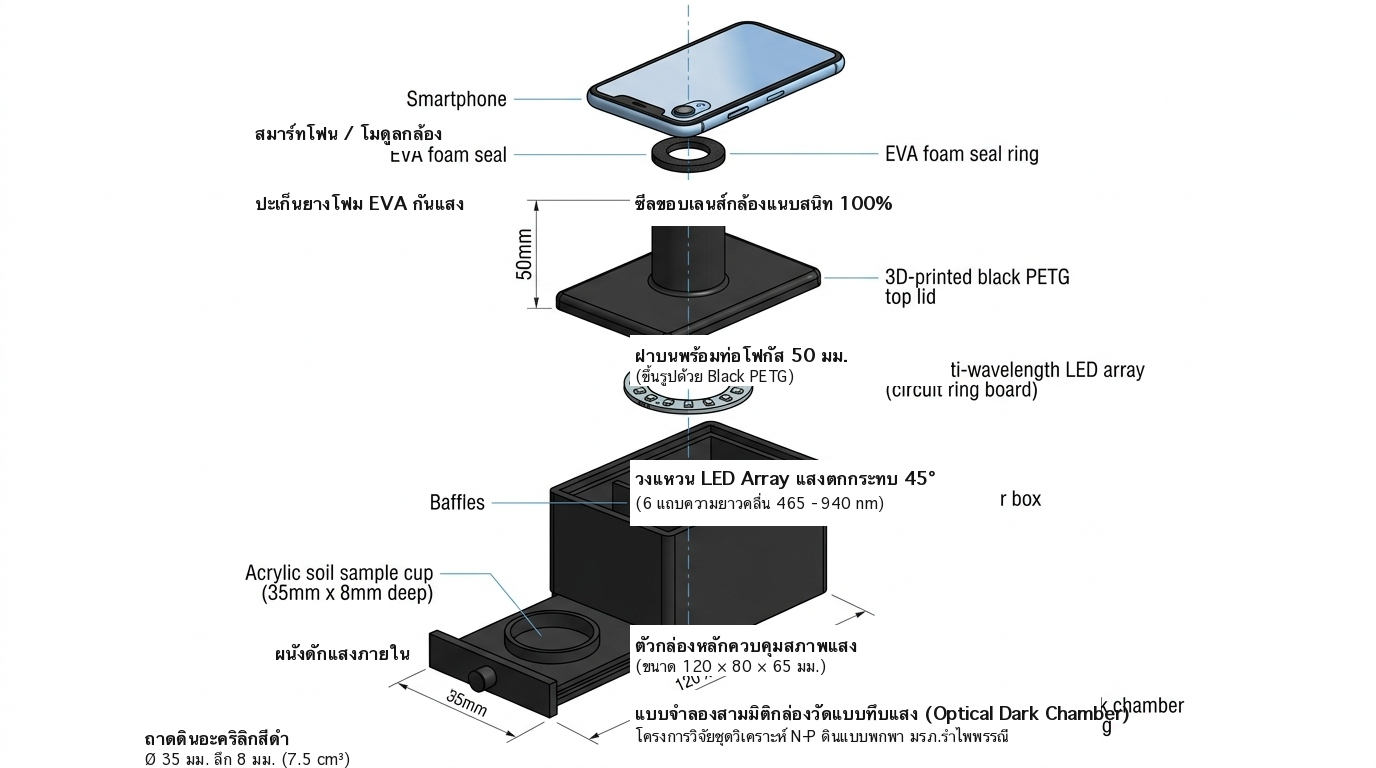
\includegraphics[width=0.78\textwidth]{figures/dark_chamber_exploded.jpg}
\caption{โครงสร้างภาพแยกชิ้นส่วนของห้องมืดควบคุมการกระเจิงแสงและระบบจัดวางหลอดกำเนิดแสงมาตรฐาน}
\label{fig:dark_chamber_exploded}
\end{figure}

\begin{figure}[H]
\centering
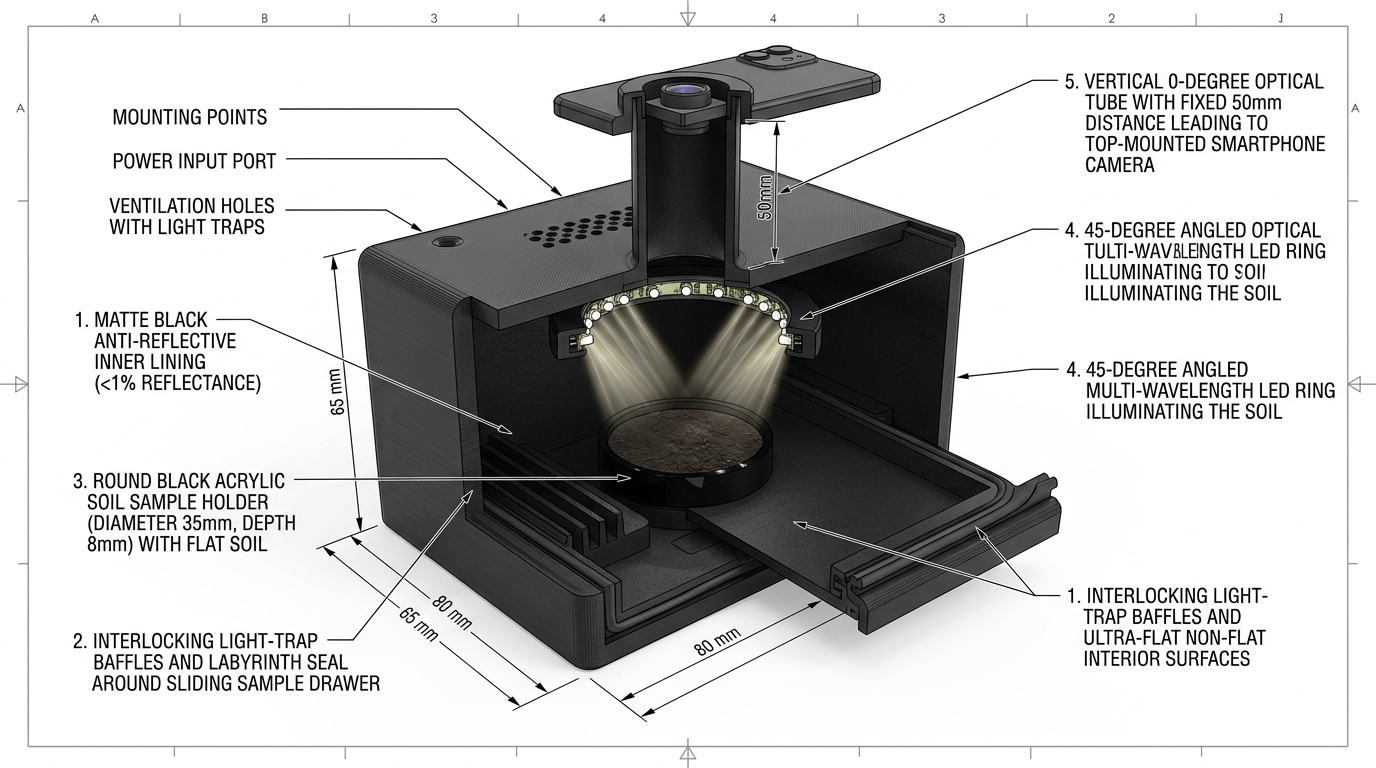
\includegraphics[width=0.78\textwidth]{figures/dark_chamber_cutaway.jpg}
\caption{มุมมองภาพตัดขวางแสดงเส้นทางเดินลำแสงตกกระทบและมุมสะท้อน 45 องศาภายในห้องมืด}
\label{fig:dark_chamber_cutaway}
\end{figure}

ห้องมืดดังกล่าวติดตั้งแหล่งกำเนิดแสงไดโอดเปล่งแสงอุณหภูมิสีคงที่ 5000 เคลวิน มีดัชนีความถูกต้องของสี (Color Rendering Index หรือ CRI) สูงกว่า 95 โดยจัดมุมการตกกระทบของแสงไว้ที่ 45 องศาเทียบกับระนาบผิวตัวอย่างดิน เพื่อลดการสะท้อนแบบแสงสะท้อนจ้า (Specular Glare) เข้าสู่เลนส์รับภาพของสมาร์ทโฟนโดยตรง และติดตั้งช่องมองภาพขนาดเส้นผ่านศูนย์กลาง 18 มิลลิเมตรที่ระนาบ 90 องศา พร้อมแผ่นกระจายแสงนาโนโพลีเมอร์ (Nano-diffuser Plate) เพื่อให้ความเข้มแสงกระจายตัวสม่ำเสมอทั่วพื้นที่ตรวจวัด ดังแสดงในภาพที่ \ref{fig:oppo_mount_setup}

\begin{figure}[H]
\centering
\begin{minipage}{0.48\textwidth}
\centering
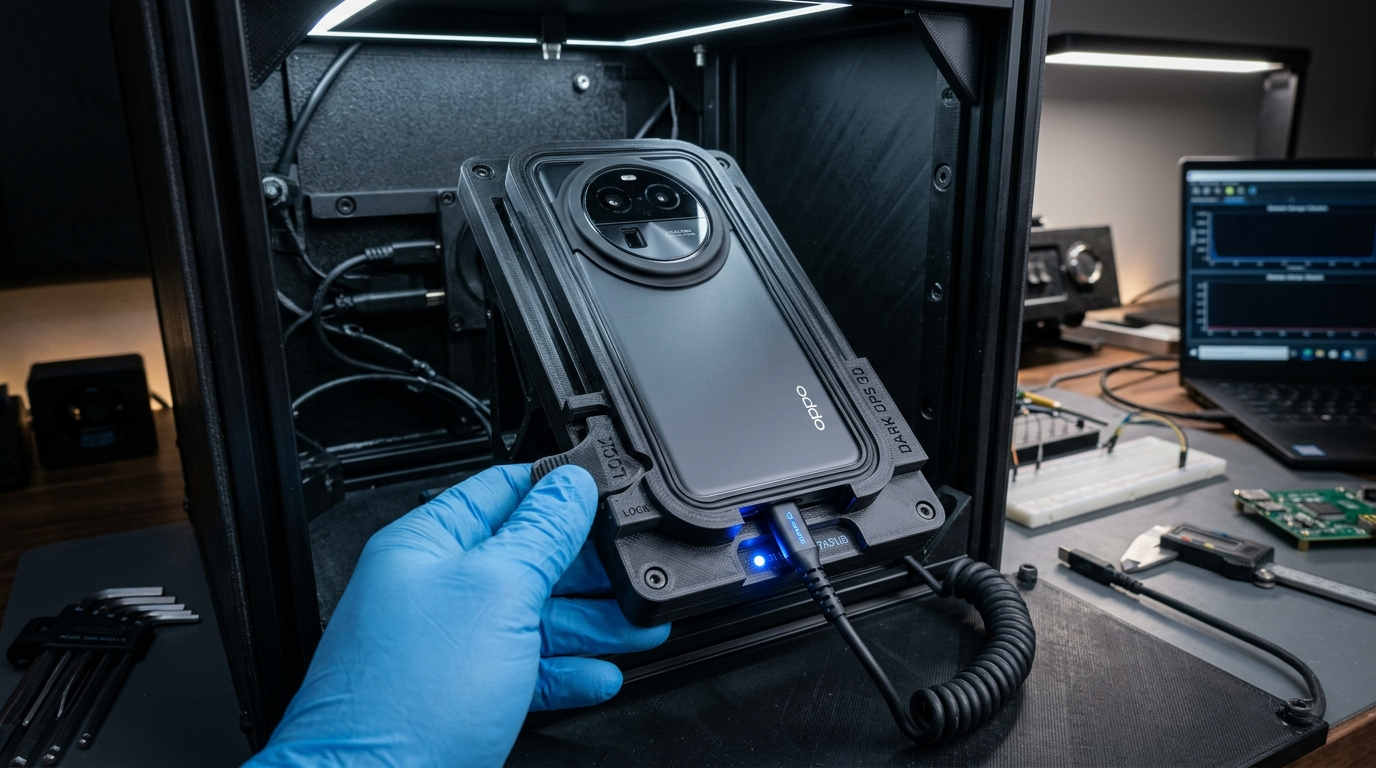
\includegraphics[width=\textwidth]{figures/oppo_macro_mount.jpg}
\end{minipage}
\hfill
\begin{minipage}{0.48\textwidth}
\centering
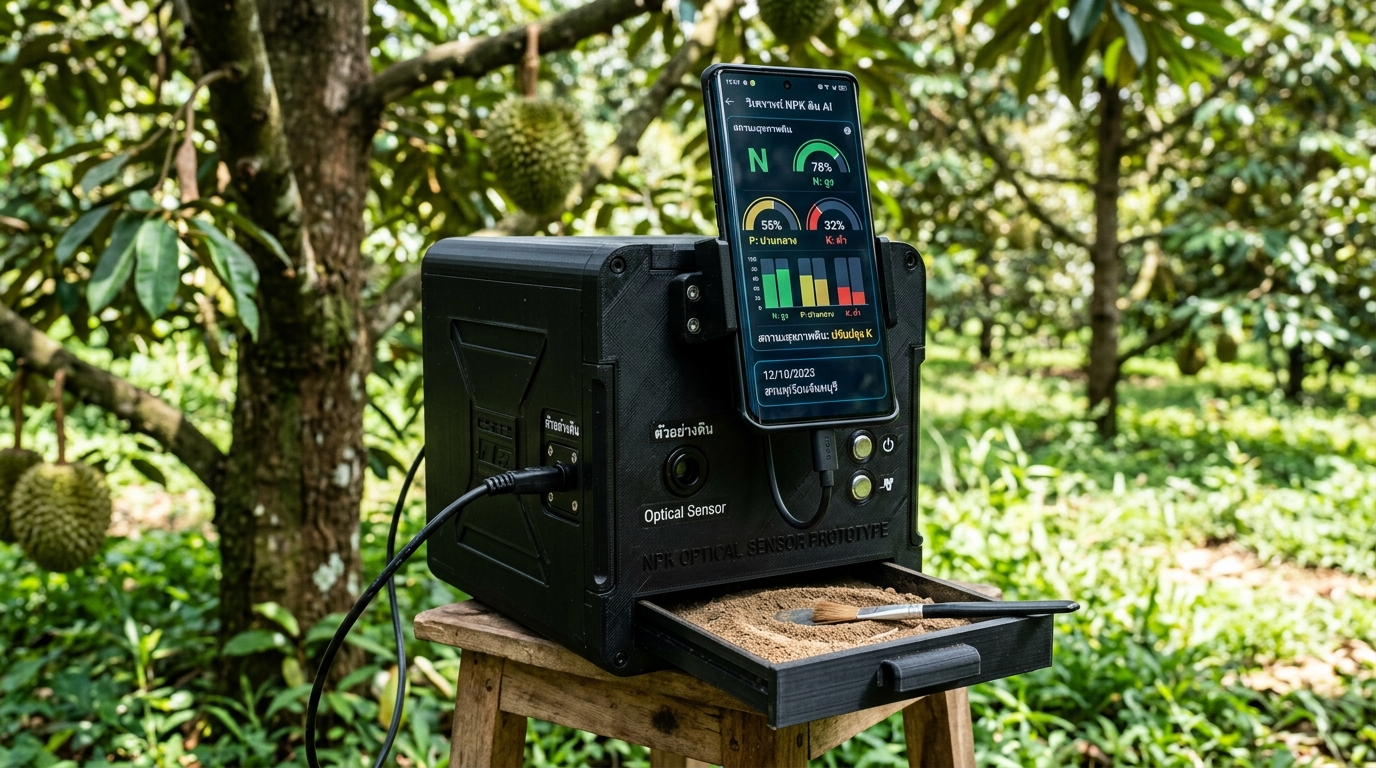
\includegraphics[width=\textwidth]{figures/oppo_npk_chamber.jpg}
\end{minipage}
\caption{ชุดแท่นยึดสมาร์ทโฟนร่วมกับห้องมืดควบคุมแสงสำหรับการวิเคราะห์คุณสมบัติดินภาคสนาม}
\label{fig:oppo_mount_setup}
\end{figure}

การออกแบบฮาร์ดแวร์ดังกล่าวทำให้ระบบสามารถเก็บรวบรวมข้อมูลภาพดิจิทัลที่มีอัตราส่วนสัญญาณต่อสัญญาณรบกวน (Signal-to-Noise Ratio, SNR) สูง ส่งผลให้โมเดลการเรียนรู้เชิงลึกสามารถสกัดคุณลักษณะสีได้อย่างมีเสถียรภาพสูงสุด
